\section{Durchführung}

    Für die Messung werden zwei Laser verwendet,
    welche monochromatisches Licht der Wellenlängen
    $\lambda = \SI{635}{\nano\meter}$ (rotes Licht) und
    $\lambda = \SI{532}{\nano\meter}$ (grünes Licht)
    erzeugen.


    \autoref{fig:aufbau_platte} zeigt den grundlegenden Versuchsaufbau.
    Die zwei Laser sind übereinander auf einer transparenten Grundplatte befestigt
    und lassen sich auf etwa einem Halbkreis um einen zentralen Punkt verschieben,
    auf dem verschiedene Objekte platziert werden können.
    Auf der transparenten Platte ist außerdem ein Reflexionsschirm angebracht,
    der auf zwei verschiedene Höhen eingestellt werden kann.\\
    Zur Messung wird die Platte auf eine Vorlage gestellt,
    welche eine Skala zeigt,
    auf welcher die zu bestimmenden Winkel abgelesen werden können.\\
    Als optische Elemente dienen ein Spiegel (Reflexionsplatte),
    eine planparallele Platte, sowie ein Prisma und Gitter verschiedener Gitterkonstanten.
    Einige dieser optischen Elemente sind in \autoref{fig:aufbau_elemente} zu sehen.

    Das optisch dünnere Medium ist bei allen Versuchen Luft.

    \begin{figure}
      \centering
      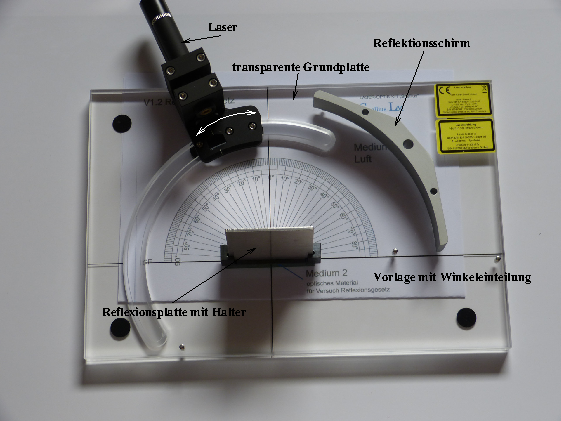
\includegraphics[width=0.8\textwidth]{content/img/Abb_3_compressed.pdf}
      \caption{Aufbau zur Untersuchung von Reflexion, Brechung und Beugung eines Lichtstrahls. \cite{versuchsanleitung}}
      \label{fig:aufbau_platte}
    \end{figure}

    \begin{figure}
        \centering
        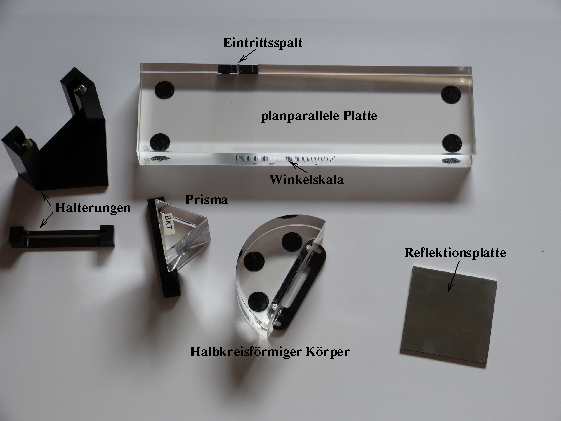
\includegraphics[width=0.8\textwidth]{content/img/Abb_4_compressed.pdf}
        \caption{Optische Elemente zur Messung von Reflexion, Brechung und Beugung. \cite{versuchsanleitung}}
        \label{fig:aufbau_elemente}
    \end{figure}


\FloatBarrier
\subsection{Untersuchung der Reflexion}

    Für diese Messung wird der Spiegel mithilfe einer Halterung in der Mitte der transparenten Platte positioniert.
    Es werden die Vorlage \textbf{A} und der grüne Laser verwendet.
    Nun wird der Laser verschoben,
    sodass der Lichtstrahl in einem Einfallswinkel $\alpha_1$ auf den Spiegel trifft.\\
    Es werden für sieben verschiedene Winkel $\alpha_1$ die Ausfallswinkel $\alpha_2$ gemessen.


\subsection{Untersuchung der Brechung}

    Diese Messung setzt sich aus zwei Teilen zusammen:
    Es wird die Brechung an einer planparallelen Platte sowie an einem Prisma untersucht.

    \begin{description}
    \item[planparallele Platte]
    \phantomsection
    \label{sec:durchfuehrung:brechung:planparallele_platte}
    Für die Messung mit der planparallelen Platte werden der grüne Laser und die Vorlage \textbf{A} verwendet.
    Beim Aufstellen der in \autoref{fig:aufbau_elemente} gezeigten Platte
    muss darauf geachtet werden,
    dass der darauf angebrachte Eintrittsspalt zum Laser hin zeigt.
    Der Brechungswinkel kann mithilfe der Skala auf der anderen Seite abgelesen werden.\\
    Es werden für sieben verschiedene Einfallswinkel $\alpha$ die Brechungswinkel $\beta$ gemessen.

    \item[Prisma]
    Für die Messung der Brechung am Prisma werden beide Laser verwendet,
    sowie die Vorlage, auf der ein Prisma-Umriss abgebildet ist.
    Das gleichseitige dreieckige Prisma wird in die Mitte der transparenten Platte gesetzt,
    wobei der Lichtstrahl auf eine der ebenen Flächen trifft.
    Gegenüber dem Laser wird eine Winkelskala aufgestellt,
    auf der auch die Lichtpunkte sichtbar gemacht werden.\\
    Es werden die Austrittswinkel $\alpha_2$ für sechs Einfallswinkel $\alpha_1$ gemessen,
    wobei $\alpha_1$ in einem Bereich von $\SI{10}{\degree} \leq \alpha_1 \leq \SI{60}{\degree}$ liegen soll.
  \end{description}


\subsection{Untersuchung der Beugung am Gitter}
\label{sec:durchfuehrung:beugung}

    Für diese Messung wird ein Gitter vor der Kante der transparenten Platte platziert,
    damit beide Laserstrahlen auf das Gitter treffen.
    Den Lasern wird eine Winkelskala von $\SI{-35}{\degree} \leq \varphi \leq \SI{35}{\degree}$ gegenübergestellt,
    auf der die Intensitätsmaxima, welche als Lichtpunkte erkennbar sind,
    abgelesen werden können.\\
    Die Messung wird mit beiden Lasern zugleich
    für die Gitter mit $\SI{600}{{Linien}\per\milli\meter}$,
    $\SI{300}{{Linien}\per\milli\meter}$ und $\SI{100}{{Linien}\per\milli\meter}$
    durchgeführt,
    wobei sich abhängig von der Anzahl der Gitterlinien
    verschieden viele Intensitätsmaxima messen lassen.
